\documentclass[%
doctor,      % тип документа
subf,        % использовать пакет subcaption для вложенной нумерации рисунков
href,        % использовать пакет hyperref для создания гиперссылок
colorlinks,  % цветные гиперссылки
%times,      % шрифт Times как основной
%fixint,     % включить прямые знаки интегралов
%classified, % гриф секретности
%facsimile,  % отображать факсимиле диссертанта
]{disser}

\usepackage[
  a4paper, mag=1000,
  left=2.5cm, right=1cm, top=2cm, bottom=2cm, headsep=0.7cm, footskip=1cm
]{geometry}

\usepackage[intlimits]{amsmath}
\usepackage{amssymb,amsfonts}
\usepackage[autostyle]{csquotes}

\usepackage[T2A]{fontenc}
\usepackage[utf8]{inputenc}
\usepackage[english,russian]{babel}
\ifpdf\usepackage{epstopdf}\fi

% Шрифт Times в тексте как основной
%\usepackage{tempora}
% альтернативный пакет (из дистрибутива TeX Live)
%\usepackage{cyrtimes}

% Шрифт Times в формулах как основной
%\usepackage[varg,cmbraces,cmintegrals]{newtxmath}
% альтернативный пакет
%\usepackage[subscriptcorrection,nofontinfo]{mtpro2}

\usepackage[style=gost-numeric,
  backend=biber,
  language=auto,
  hyperref=auto,
  autolang=other,
  sorting=none
]{biblatex}

\addbibresource{thesis.bib}

% Номера страниц снизу и по центру
%\pagestyle{footcenter}
%\chapterpagestyle{footcenter}

% Точка с запятой в качестве разделителя между номерами цитирований
%\setcitestyle{semicolon}

% Ссылки на работы соискателя включаются в общий список литературы
\let\citemy=\cite

% Использовать полужирное начертание для векторов
\let\vec=\mathbf

% Путь к файлам с иллюстрациями
\graphicspath{{fig/}}

\begin{document}

% Переопределение стандартных заголовков
%\def\contentsname{Содержание}
%\def\conclusionname{Выводы}
%\def\bibname{Литература}

% Включение файла с общим текстом диссертации и автореферата
% (текст титульного листа и характеристика работы).

\mkcommonsect{actuality}{������������ ������}{%
����� �������
}

\mkcommonsect{objective}{���� ��������������� ������}{%
����� �������
}

\mkcommonsect{novelty}{������� �������}{%
����� �������
}

\mkcommonsect{value}{������������ ��������}{%
����� �������
}

\mkcommonsect{results}{%
�� ������ ��������� ��������� �������� ���������� � ���������:}{%
����� �������
}

\mkcommonsect{approbation}{��������� ������}{%
����� �������
}

\mkcommonsect{pub}{����������}{%
����� �������
}

\mkcommonsect{contrib}{������ ����� ������}{%
����� �������
}

\mkcommonsect{struct}{��������� � ����� �����������}{%
����� �������
}


% номер копии для грифа секретности
%\copynum{1}
% класс доступа
%\classlabel{Для служебного пользования}

% номер УДК
\libcatnum{12345}

\title{ДИССЕРТАЦИЯ\\
на соискание ученой степени\\
доктора физико-математических наук}

\maketitle

%%
%% Titlepage in English
%%
%
%\institution{Name of Organization}
%
%\title{Doctoral Dissertation}
%
%% Topic
%\topic{Dummy Title}
%
%% Author
%\author{Author's Name}
%
%\specnum{01.04.05}
%\spec{Optics}
%
%%\specsndnum{01.04.07}
%%\specsnd{Condensed matter physics}
%
%% Scientific consultants
%\scon{B.\,B.~Baranov}
%\sconstatus{Professor}
%%\sconsnd{P.\,P.~Petrov}
%%\sconsndstatus{Professor}
%
%% City & Year
%\city{Saint Petersburg}
%\date{\number\year}
%
%\maketitle[en]

% Содержание
\tableofcontents

% Введение
\intro

%
% ������������ ����� ������� ������������ � ����� common.tex.
%

% ������������ ������
\actualitysection
\actualitytext

% ���� ��������������� ������
\objectivesection
\objectivetext

% ������� �������
\noveltysection
\noveltytext

% ������������ ��������
\valuesection
\valuetext

% ���������� � ���������, ��������� �� ������
\resultssection
\resultstext

% ��������� ������
\approbationsection
\approbationtext

% ����������
\pubsection
\pubtext

% ������ ����� ������
\contribsection
\contribtext

% ��������� � ����� �����������
\structsection
\structtext

% Обзор литературы
%\input{review}

% Основная часть
%% Глава 1
\chapter{�������� �����}
\section{�������� ������}

��������������� ������� $\frac{1}{\epsilon^*}=\frac{1}{\epsilon_\infty}-\frac{1}{\epsilon_0}$.
��������������� ������� � ����� ���������� $\dfrac{1}{\epsilon_\infty}$.
������ �� ����������~\cite{Efros-1982-FTP16-82-1209,%
Yoffe-1993-AP-42-173,Kayanuma-1988-PRB-38-9797,Segall-1968}.
������ �� �������~\eqref{eq:e}
\begin{equation}\label{eq:e}
  \vec P=\sqrt{\frac{N_0 m_r \Omega_{LO}}{4\pi\epsilon^*}}(\vec u_+ - \vec u_-).
\end{equation}

������ �� ���.~\ref{fig:f}
\begin{figure}[!ht]
\centering
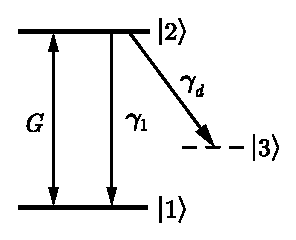
\includegraphics[width=4cm]{fig}
\caption{\label{fig:f}%
������� � �������.
}
\end{figure}

\begin{wrapfigure}{r}{0.35\textwidth}
  \centering
  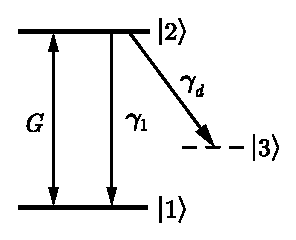
\includegraphics[width=4cm]{fig}
  \caption{\label{fig:ff}������� <<� ������>>.}
\end{wrapfigure}

���� �������� ������� ����������-�������� ������� $E_2-E_1$ ������ � ������� ����������� ����������� ������ $\hbar\Omega_{LO}$, �� � ���������� �������� ������� ������� ������������� ����� ������������ ������� ������������ ��� ���� ���������, �� ����������� ������� �� �������� � $E_2$. �������� ������� ��������� ������������ ����� ��������� ���������� ����� ����������� ���������.

������ �� �������~\ref{tab:t1}.
\begin{table}[!ht]
  \centering
  \caption{������ �������}\label{tab:t1}
  \vskip1.em
  \begin{tabular}{l|ccc}
    \hline\hline
    & \quad$\lambda \times 10^{-11}$,~$\text{���}\cdot\text{��}^{-2}$\quad &
    \quad$\mu \times 10^{-11}$,~$\text{���}\cdot\text{��}^{-2}$ & \quad$\rho$, $\text{�}\cdot \text{��}^{-3}$\quad \\
    \hline
    InP       & 3.82 & 1.69 & 4.14 \\
    SiO$_{2}$ & 1.57 & 3.11 & 2.2  \\
    \hline\hline
  \end{tabular}
\end{table}

\begin{figure}[!ht]
\centering
  \begin{minipage}{5cm}
    \centering
    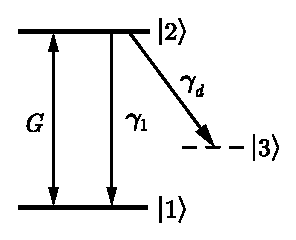
\includegraphics[width=4cm]{fig}
    \caption{������� � ��������� ���������}
  \end{minipage}
  \quad
  \begin{minipage}{5cm}
    \centering
    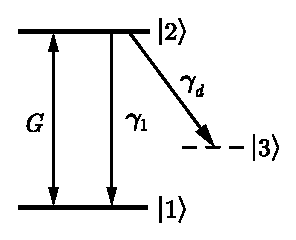
\includegraphics[width=4cm]{fig}
    \caption{������� � ��������� ���������}
  \end{minipage}
  \quad
  \begin{minipage}{5cm}
    \centering
    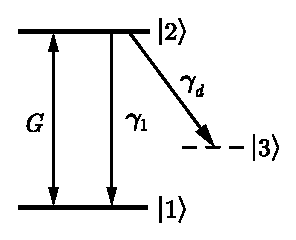
\includegraphics[width=4cm]{fig}
    \caption{������� � ��������� ���������}
  \end{minipage}
\end{figure}

\begin{figure}[!ht]
\centering
  \begin{minipage}{5cm}
    \centering
    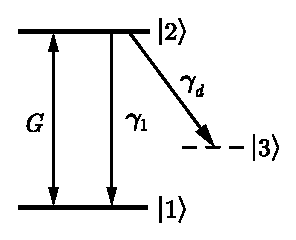
\includegraphics[width=4cm]{fig}
  \end{minipage}
  \quad
  \begin{minipage}{5cm}
    \centering
    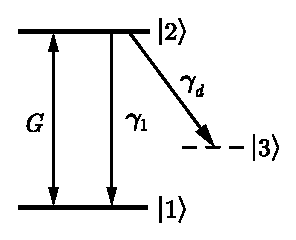
\includegraphics[width=4cm]{fig}
  \end{minipage}
  \caption{������� � ������ ���������}
\end{figure}

������ �� ���������� ������� (���.~\ref{fig:sub1})

\begin{figure}[!ht]
\centering
  \subfloat[][]{\label{fig:sub1}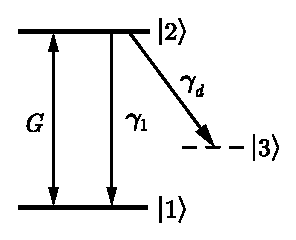
\includegraphics[width=4cm]{fig}}\quad
  \subfloat[][]{\label{fig:sub2}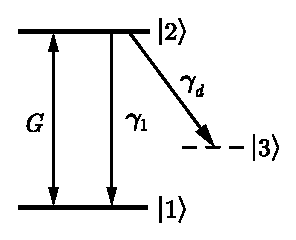
\includegraphics[width=4cm]{fig}}\quad
  \subfloat[][]{\label{fig:sub3}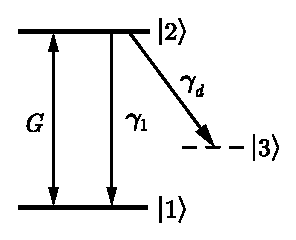
\includegraphics[width=4cm]{fig}}
\caption[]{%
������� � ������ ��������� � ����������� ����������:
  \subref{fig:sub1} ������ 1,
  \subref{fig:sub2} ������ 2,
  \subref{fig:sub3} ������ 3.
}
\end{figure}

\subsection{�������� ���������}
����� ���������
\subsubsection{�������� ���-���������}
����� ���-���������
\paragraph{�������� ���������.}
����� ���������
\subparagraph{�������� ������������.}
����� ������������

������������ ��������� ������������� ��������� ���� <<�������>>.

\newtheorem{lemm}{�����}[chapter]

\def\thelemmstyle{\bf}
\def\oparglemmstyle{}
\def\lemmstyle{\it}
\def\preoparglemm{\{}
\def\postoparglemm{\}}

\newtheorem{remark}{����������}[chapter]

\def\remarkstyle{\it}
\def\theremarkstyle{}
\def\posttheremark{:}

\begin{lemm}[����]
�������, ������������� �� ����� ��������� ������������� �������������, ������ ���������.
\end{lemm}

\begin{remark}
������� � ���� ���������� �������.
\end{remark}

%% Глава 2
%\input{2}

% Заключение
\input{concl}

% Список сокращений и условных обозначений
%% Список сокращений и условных обозначений
\defs

\begin{longtable}{lp{0.025\textwidth}p{0.89\textwidth}}
$\vec A$ & --- & векторный потенциал\\
$I$ & --- & интенсивность света\\
$j_l$ & --- & сферическая функция Бесселя первого рода\\
$Y_{lm}$ & --- & сферическая гармоника\\
\end{longtable}


% Словарь терминов
%% ������� ��������
\dict

\textbf{������} "--- �����������.


% Список литературы
\printbibliography[heading=bibintoc]

% Список иллюстративного материала
%\listoffigures

% Приложения
%\appendix
%\input{app-a}

\end{document}
